\clearpage % clear the prior chapter's page

\chapter{Efficient sampling of loop conformations using conformational hashing and random coordinate descent} \label{app:loophash}
%\vspace{-7mm}
%\bigskip

The contents of this Appendix have been previously published \citep*{DelAlamo2021}.

%\vspace{-7mm}
\bigskip

\emph{De novo} construction of loop regions is an important problem in computational structural biology. Compared to regions with well-defined secondary structure, loops tend to exhibit significant conformational heterogeneity. As a result, their structures are often ambiguous when determined using experimental data obtained by crystallography, \gls{cryoem}, or \gls{nmr}. Although structurally diverse models could provide a more relevant representation of proteins in their native states, obtaining large numbers of biophysically realistic and physiologically relevant loop conformations is a resource-consuming task. To address this need, we developed a novel loop construction algorithm, Hash/RCD, that combines knowledge-based conformational hashing with \gls{rcd}. This hybrid approach achieved a closure rate of 100\% on a benchmark set of 195 loops in 29 proteins that range from three to thirty-one residues. More importantly, the use of templates allows Hash/RCD to maintain the accuracy of state-of-the-art coordinate descent methods while reducing sampling time from over \SI{400}{ms} to \SI{141}{ms}. These results highlight how the integration of coordinate descent with knowledge-based sampling overcomes barriers inherent to either approach in isolation. This method may facilitate the identification of native-like loop conformations using experimental data or full-atom scoring functions by allowing rapid sampling of large numbers of loops. In this manuscript, we investigate and discuss the advantages, bottlenecks, and limitations of combining conformational hashing with \gls{rcd}. By providing a detailed technical description of the Hash/RCD algorithm, we hope to facilitate its implementation by other researchers.

\section{Introduction}\label{sec:loophash_intro}

Despite its importance to computational structural biology, the prediction of protein loops remains a challenge \citep*{Li2013}. Without the periodic backbone hydrogen bonds defining regular secondary structure, a large conformational space needs to be searched. Moreover, loops can interconvert between many isoenergetic conformations, complicating efforts to identify a single conformation at a global energy minimum. Perturbation of loops in structures determined using experimental techniques such as crystallography further complicates the development of loop modeling methods \citep*{Jacobson2004}, as the conformations observed in a crystal lattice may be artifacts of experimental design and/or data collection.

Algorithms that predict loop regions in proteins generally use one of several strategies. Template-based methods rely on experimentally determined loop conformations deposited in the Protein Databank to build missing loop regions. For example, in the Loophash algorithm \citep*{Tyka2012}, which is implemented in Rosetta \citep*{Leaver-fay2011, Leman2020}, the sequence of the loop target is threaded onto a template selected from a loop library. Other examples of template-based methods include Superlooper \citep*{Hildebrand2009}, which searches the Loops-in-proteins database \citep*{Michalsky2003}; FREAD \citep*{Choi2010}, which uses several criteria to identify experimentally determined loops of interest; and DaReUs-Loop \citep*{Karami2018, Karami2019}, which uses loop flanking regions to identify suitable candidate loops for modeling. In general, template-based loop prediction has the advantage of being fast, since the loop dihedral angles have been experimentally observed. However, they are limited by the underrepresentation of long loops in the PDB (11 or more residues), which leads to fewer templates. Consequently, this approach is generally suitable for short and medium-sized loops (10 or fewer residues).

An alternative approach for modeling missing loops is to do so \emph{de novo}. This approach achieves loop closure by relying on an energy function to optimize the dihedral angles of the residues comprising the loop. Various methods have been described that use this strategy, such as GalaxyLoop-PS2 \citep*{Park2014}, ModLoop \citep*{Fiser2000}, LEAP \citep*{Liang2014}, PETRA \citep*{Deane2000}, and Rosetta-KIC \citep*{Mandell2009} and NGK \citep*{Stein2013}. A widely-used method is the \gls{ccd} algorithm \citep*{Canutescu2003, Boomsma2005}, which was inspired by the random tweak algorithm used in robotics. Both \gls{ccd} and the closely-related \gls{rcd} algorithm \citep*{Chys2013} rotate the loop’s backbone torsion angles to place the a "virtual" terminal residue over the loop’s anchor point. Coordinate descent methods have the advantage of high closure rates, even among longer loops. However, as with all \emph{de novo} methods, they are limited by their time complexity, which depends on the loop's sequence length. Moreover, they can introduce distortions in the loop’s dihedral angles.

Finally, a series of “hybrid” approaches hold promise to find middle ground between low time complexity of template-based modeling with the high closure rate of \emph{de novo}-based methods. For example, both CODA \citep*{Deane2001} and Sphinx \citep*{Marks2017} arrive at consensus predictions by combining the template-based predictions from FREAD \citep*{Choi2010} with loops modeled \emph{de novo}. The comparative modeling protocol RosettaCM \citep*{Song2013} predicts loop conformations by assembling three- and nine-residue fragments from the PDB and closing loop regions using Cartesian minimization. Similar protocols have used a hybrid approach to model long hypervariable loops in antibodies \citep*{Fasnacht2014, Martin1989, Mas1992, Whitelegg2000}. In summary, these methods allow long loops to be predicted in a reasonable amount of time without being restrained by the lack of experimentally determined templates of a given length.

An optimal loop construction algorithm would find the middle ground between low time complexity and high closure rate. Here we introduce and discuss an algorithm, Hash/RCD, that combines conformational hashing with \gls{rcd}. Hash/RCD circumvents the lack of templates for long loops by constructing them from shorter fragments using a \gls{mc} framework. The resulting hybrid algorithm, which is implemented as part of the \gls{bcl} \citep*{Karakas2012, Woetzel2012}, combines the advantages of conformational hashing and coordinate descent while mitigating their respective limitations. 

This Appendix discusses the implementation and performance of conformational hashing with and without \gls{rcd} and is organized as follows. First, Materials and Methods (section \ref{sec:loophash_methods}) describes the general methodology that combines conformational hashing and \gls{rcd} within an \gls{mc} framework. Next, generation of the loop template library is discussed. This is followed by the mathematical details regarding the parametrization of 1) loop conformations for conformational hashing and 2) fragments for recombination into longer loop templates. We then provide a technical description of the \gls{rcd} method used in this study and a summary of the benchmark set used to quantify the performance of Hash/RCD. Finally, this section is concluded with a description of the method's performance compared to the Rosetta Loophash algorithm \citep*{Tyka2012}, \gls{rcd} in isolation, and the orthogonal sampling approach RosettaCM \citep*{Song2013}. In the Results section we discuss the performance of Hash/RCD, which we evaluated using several metrics, including closure rate and \gls{cpu} time consumption. We also explored the limits of conformational hashing and compare the loops generated by Hash/RCD to those generated by Rosetta Loophash, \gls{rcd} in isolation, and RosettaCM.

\section{Materials and Methods}\label{sec:loophash_methods}

\subsection{General methodology and generation of the loop template library}

The sampling approach used by Hash/RCD is described in Figure \ref{fig:loophash_db} and consists of two stages and a post-processing step. The first stage uses conformational hashing to construct loop regions from precomputed templates (the term “template” refers to any experimentally determined loop structure used for modeling purposes). The second stage identifies and closes loops that could not be closed during the first stage using \gls{rcd}. Finally, a post-processing step constructs loops that may be missing from the protein's N- and C-termini.

\begin{figure}[h]
\centering
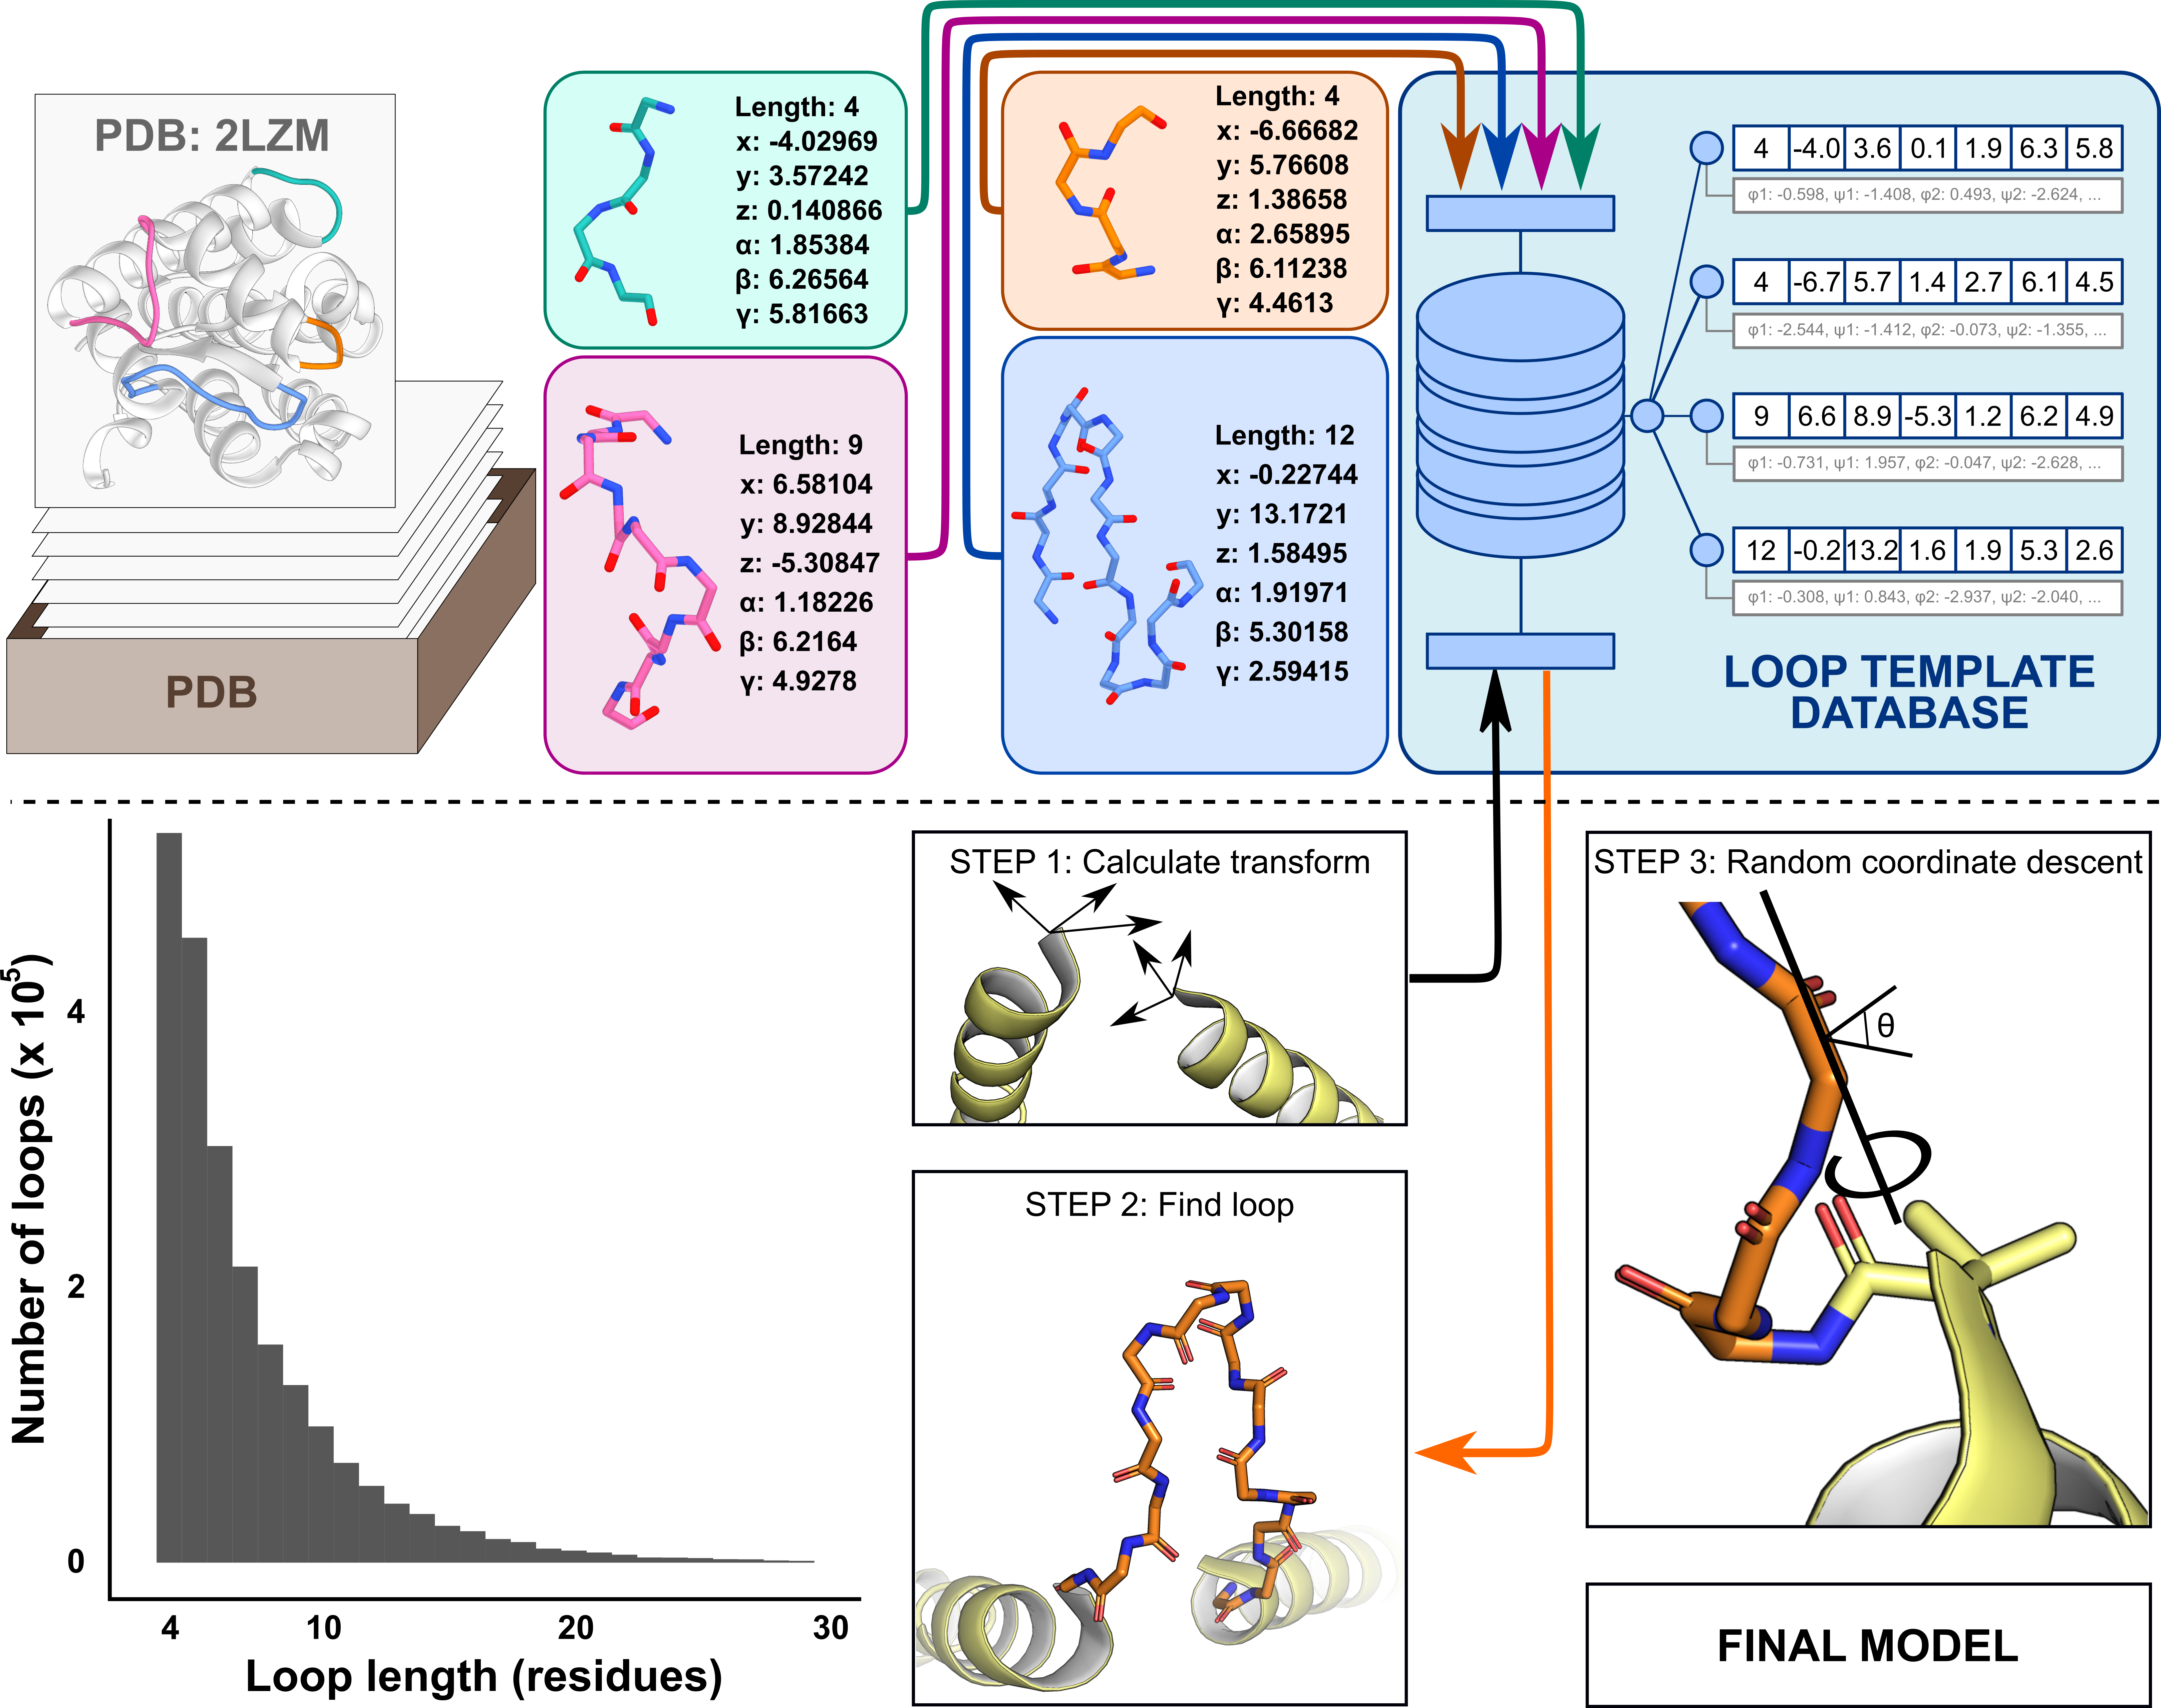
\includegraphics[width=6in]{Figures/loophash_db.pdf}
 \caption[Overview of the Hash/RCD algorithm.]{Overview of the Hash/RCD algorithm. Top: Loop parameterization using a hash key computed from the length and relative orientation of its anchor points. A hash look-up identifies and selects suitable template conformations. Bottom left: The initial template library consisted of about 3.7 million loop conformations with different sequence lengths. These loops were collected from a set of about 87,000 protein structures deposited in the PDB. Bottom right: Depiction of the conformational hashing and \gls{rcd} stages of this algorithm. An \gls{mc} framework embeds both stages and allows loop templates to be added, replaced, and removed.}
\label{fig:loophash_db}
\end{figure}

We compiled the initial template library used by the first stage from a nonredundant subset of experimentally determined structures in the PDB \citep*{Bernstein1978}. The Dunbrack lab’s protein sequence culling server (PISCES) server was used to filter out structures whose resolutions exceeded \SI{3.0}{\angstrom} and did not fully or partially consist of $\mathrm{C_{\upalpha}}$-traces \citep*{Wang2003, Wang2005}. This avoided the overrepresentation of protein structures that have been determined in multiple nearly identical conformations and resulted in about 87,000 structures. From there, we discarded the \gls{sse} definitions provided in the PDB files, instead using the \gls{sse} definition program \gls{dssp} \citep*{Kabsch1983}. Loops were defined as contiguous regions in sequence space that could not assigned any regular secondary structure. This approach both ensured reproducibility and standardized the assignment of secondary structure on the basis of backbone hydrogen bonding geometry. Finally, we removed loops containing unresolved backbone coordinates. Using this approach, we collected about 3.7 million loop conformations (Figure \ref{fig:loophash_db}).

The templates were then translated into hash keys describing the geometric aspects of the anchor residues flanking the loop (see next section for details). Lists of loops corresponding to specific geometries were stored together in a hash table. As we discuss below, Hash/RCD draws from this hash table to sample the addition and replacement of loops for given protein models by computing the parametrization of the missing loop, calculating the associated hash key, and inserting a suitable template chosen at random. The loop's sequence is then threaded over this template and inserted into the protein model. By relying on a hash table to identify templates, this approach has the advantage of $O(1)$ computation time and generally requires \gls{cpu} time on the order of microseconds. Since long loops have fewer templates in the loop library, they could be assembled from shorter fragments using a procedure discussed below.


Following conformational hashing, Hash/RCD uses random coordinate descent, previously described by Canutescu et al. \citep*{Canutescu2003} and Chys and Chacon \citep*{Chys2013}, to minimize the distance between a moving (loop end) and target (anchor) set by calculating the rotation that must occur around a given axis $({\phi},{\psi})$. We took several steps to diversify the loops generated this way. First, we found that randomly choosing which dihedral angle (either $\phi$ or $\psi$) at every step allowed Hash/RCD to avoid getting stuck in non-closable conformations. Additionally, only a random fraction of the rotation is applied. Further, we modified the original protocol to bend the terminal regions of the \gls{sse}s flanking the loop (Figure \ref{fig:loophash_db}). Finally, supplementing this protocol with scoring functions allows it to identify and reject rotations that cause the loop to clash with the rest of the protein model.

The final step of the protocol constructs the terminal loop regions. These were initialized with dihedral angles that are randomly chosen from a $({\phi},{\psi})$ distribution derived from experimentally determined protein structures. The coordinate descent algorithm was then executed to resolve steric interferences and/or energetically unfavorable configurations.

\subsection{Parametrization of loop conformations and selection of suitable conformations}

In addition to their length, loop conformations can be defined by the relative rotational and translational orientation of the anchor residues flanking them. Therefore, we defined a local orthonormal coordinate system for the anchor points of each loop as $(e_x, e_y, e_z)$ based on their backbone coordinates. Here $e_x$ is the normalized $C_{\upalpha}-C$ vector, $e_y$ is the normalized component of the $C_{\upalpha}-O$ vector orthogonal to $e_x$, and $e_z$ is computed from $e_x$ and $e_y$ such that $e_z=e_x×e_y$. Accordingly, the translation vector resides within this coordinate system and is defined as follows: 

\begin{equation}
    \vec{t}=(t_{\mathup{x}},t_{\mathup{y}},t_{\mathup{z}} )=(\alpha_{\mathup{c,x}}-\alpha_{\mathup{n,x}},\alpha_{\mathup{c,y}}-\alpha_{\mathup{n,y}},\alpha_{\mathup{c,z}}-\alpha_{\mathup{n,z}})
\end{equation}

Here $\alpha_{\mathup{c,x}}$ and $\alpha_{\mathup{n,x}}$ are the $x$-coordinates of the $C_{\mathup{\upalpha}}$-atom of the N-terminal and C-terminal anchors, respectively. The relative rotational orientation of the two anchor points was quantified using Euler angles $(\alpha,\beta,\gamma)$ following the extrinsic $x$-$y$-$z$ convention \citep*{Pio1966}. These can be readily extracted from the matrix $\mathbf{M}_{\mathup{r}}$ describing the rotation between both coordinate systems that can be computed as $\mathbf{M}_{\mathup{r}}=\mathbf{M}_{\mathup{n}}^{-1}\cdot \mathbf{M}_{\mathup{c}}$, where $\mathbf{M}_{\mathup{n}}$ and $\mathbf{M}_{\mathup{c}}$ are the transformation matrices of the local coordinate systems at the N- and C-terminal anchor points \citep*{Slabaugh1999}.

Thus, each loop was parametrized into seven parameters: the loop's sequence length ($d$), translation vector $(t_{\mathup{x}},t_{\mathup{y}},t_{\mathup{z}})$, and Euler angles $(\alpha,\beta,\gamma)$. Each parameter is discretized into bins and translated into a one-dimensional hash key $k$ using the hash function $f$:

\begin{equation}
    f:d×(t_{\mathup{x}},t_{\mathup{y}},t_{\mathup{z}} )×(\alpha,\beta,\gamma)\rightarrow k
\label{eq:loophash_hashfxn}
\end{equation}

By grouping structurally similar loops into the same bins using this function, sparse populations within the hash map are avoided. We evaluated several different bin sizes in this study and found bin sizes of \SI{1}{\angstrom} for the translation vector and 60° for the Euler angles provided the optimal balance between closure rates and accuracy. Additionally, the hash map only stores the dihedral angles $(\phi, \psi)$ of each residue in the loop conformation. As a result, each loop conformation $c$ can be described using only $2d+2$ parameters, e.g. $c=(\psi_{\mathup{N}},\phi_{1},\psi_1,…,\phi_d,\psi_d,\psi_{\mathup{C}})$. Here $d$ is the length of the loop in amino acid residues, $\psi_{\mathup{N}}$ is the $\psi$-angle of the N-terminal anchor point, $(\phi_{\mathup{i}},\psi_{\mathup{i}})$ are the dihedral angles of the $i$th residue of the loop, and $\phi_C$ is the $\phi$-angle of the C-terminal anchor point. The key-value pair $(k,c)$ of each conformation is stored in the hash map accordingly.

These steps are all carried out during the generation of the loop template prior to loop prediction. During modeling, loop look-up proceeds as follows. First, the coordinate systems for the anchor points are computed and converted into a hash function (Equation \ref{eq:loophash_hashfxn}). Second, a range of suitable conformations capable of closing this loop are returned in $O(1)$ time, and one is chosen at random. Third, the sequence of the loop being modeled is threaded onto this randomly chosen conformation, a process that happens in $O(n)$ time. Therefore, the overall time complexity of the algorithm is limited by the linear-time computation of this last step, which is in turn determined by the length of the loop being modeled.

\subsection{Integration of conformational hashing within a Monte Carlo Metropolis framework}

In a protein model containing multiple loop regions, closing a certain loop with a certain conformation might hinder the closure of other loops. Consequently, our algorithm must be able to sample different combinations of loops without needlessly increasing computational complexity. Owing to the previously demonstrated success of \gls{mc} algorithms \citep*{Leaver-fay2011, Leman2020, Karakas2012, Fischer2016a}, we embedded the conformational hashing step in an \gls{mc} framework. Effectively, the loop construction algorithm consists of two sub-algorithms, conformational hashing and \gls{rcd}, which are executed back-to-back. Each sub-algorithm places a "pseudo-residue" at the terminal end of a loop and tries to perfectly superimpose it over the corresponding anchor residue. Loop closure is calculated using the \gls{rmsd} of this pseudo-residue and the anchor residue; we use an \gls{rmsd} cutoff of \SI{0.08}{\angstrom} to account to allow for minor inaccuracies in bond lengths and angles.

In the \gls{mc} implementation of the conformational hashing algorithm (Figure \ref{fig:loophash_db}), a loop is randomly selected, perturbed, and evaluated using a scoring function. Several perturbations can be sampled. First, missing loops can be added directly from the hash map. Second, subregions of a loop can be replaced with loops added from the hash map. Third, short stretches of up to three residues can be cut back at the anchor residues and replaced with loop conformations obtained from the hash map. Fourth, when suitable loops with sequence length $d+2$ are absent from the template library, stepwise construction of loops can instead be achieved by randomly selecting loop conformations with sequence length less than $d-2$ from the template library and applying them to the selected template.

Depending on the impact of these perturbations on the score of the model, the new model is either accepted or rejected \citep*{Karakas2012}.  Knowledge-based score terms used to evaluate loop conformations include clash evaluation, consistency with Ramachandran potentials, and residue-residue interactions. We also added score terms to evaluate a model's consistency with secondary structure prediction algorithms such as PSI-blast based secondary structure Prediction \citep*{Jones1999, Ward2003}, Jufo9D \citep*{Leman2013}, and MASP \citep*{Mendenhall2014}. Finally, a score term consisting of 30\% of the scoring function pushes the algorithm toward loop closure by linearly penalizing stretches of missing residues.

\subsection{Construction of missing loop regions using random coordinate descent}

The \gls{rcd} algorithm closed loops only when they could not be closed using the conformational hashing algorithm. Its implementation is modeled on the CCD algorithm described by Canutescu et al. \citep*{Canutescu2003}, which is in turn based on the random tweak algorithm \citep*{Fine1986, Shenkin1987}; additionally, we included several modifications discussed by Chys and Chacon \citep*{Chys2013}. This portion of the algorithm can be divided into a pre-stage and a main-stage component.

During the pre-stage, missing residues are dynamically added to the anchor residues. The backbone dihedral angles of these residues are initialized with $(\phi, \psi)$ angles derived from a probability distribution of experimentally observed backbone dihedral angles. Then, using a knowledge-based potential, these $(\phi, \psi)$ angles are subsequently perturbed and evaluated. Potential inaccuracies in the secondary structure prediction are accounted for by adding and/or removing residues from the anchor \gls{sse}s. Throughout this pre-stage, sampling is guided by scoring terms evaluating the completeness of the amino acid sequence, steric interference between residues, residue-residue interactions, and the loop trajectory towards its anchor point. This module also constructed the terminal loop regions of the protein models. The main-stage portion of the algorithm iteratively uses \gls{rcd} to calculate the rotation that must occur around a given axis ($\phi$ of $\psi$) to minimize the distance between the end of the loop and the target coordinates over many iterations to close a chain break. Throughout this step, residue-residue interactions and steric interferences between residues were evaluated using scoring functions.

We found that running the conformational hashing algorithm for 500 iterations appeared to offer the best balance between performance (loop closure) and time complexity. The algorithm could be terminated early if no score improvements were identified after 50 iterations. For the \gls{rcd} algorithm, we obtained the best results when the algorithm was run for 2000 total iterations with the option of terminating early after 500 iterations without any improvements.

\subsection{Compensation for lack of templates for long loops}

The initial set of about 87,000 protein structures contained about 3.7 million loop templates. Of those, the majority of these templates (about 2.2 million) were four or more residues in length (Figure \ref{fig:loophash_db}). By contrast, only 12\% of the templates were ten or more residues in length. Moreover, longer loops cover a greater conformational space, making the conformational hashing algorithm less likely to close these loops. We developed a two-pronged approach to overcome this challenge.

First, we supplemented our algorithm with a method that combines two short loop templates into a larger loop template by superimposing the backbone coordinates of one loop's C-terminal anchor point with the backbone coordinates of the other loop's N-terminal anchor point. The resulting template has a sequence length of $d=d_1+d_2+1$, with $d_n$ being the sequence length of the $n$th template. The translation vector $\vec{t}$ and the Euler angles $(\alpha,\beta,\gamma)$ are then computed in a straightforward manner. The local coordinate system of the N-terminal anchor point of the second template is first transformed into the local coordinate system of the N-terminal anchor point of the first template. This is achieved by multiplying the first coordinate system's rotation matrix the inverse of the second coordinate system's rotation matrix, i.e., $\mathbf{M}=\mathbf{M}_2^{-1}\cdot \mathbf{M}_1$. By multiplying the translation vector $t_2$ of the second template with this matrix, the resulting translation vector can be computed by simple vector addition, i.e., $\vec{t}=t_1+(t_2\cdot \mathbf{M})$.

Nevertheless, although this approach is theoretically sound, we found that small inaccuracies, likely due the binning strategy used in the original hash map, could be propagated when templates generated this way are in turn combined into new templates. Therefore, the stored dihedral angles for both templates were recombined into a sequence consisting of $2(d_1+d_2+2)$ dihedral angles: $(\psi_{n,1},\phi_1,1,\psi_1,1,…,\phi_{1,d},\psi_{1,d},\phi_{1,\mathup{c}},\psi_{\mathup{n},2},\phi_2,1,\psi_2,1,…,\phi_{2,d},\psi_{2,d},\phi_{2,\mathup{c}})$. An artificial amino acid sequence of length $d+2$ was generated within the algorithm and fitted against the combined sequence of dihedral angles, permitting the accurate computation of this template's parameterization. 

\subsection{The benchmark set used to evaluate the algorithm}

We evaluated the performance of this algorithm using a benchmark set consisting of twenty-nine soluble and membrane proteins (Table \ref{tab:loophash_benchmark}). This included the set of soluble proteins previously used by Tyka et al. to benchmark the Rosetta Loophash algorithm \citep*{Tyka2012}, as well as the eleven membrane proteins previously used to benchmark the protein structure prediction algorithm BCL::MP-Fold \citep*{Fischer2015}. These proteins ranged in size from 57 to 1,560 residues with varying $\alpha$-helical and $\beta$-strand secondary structure content. The 195 loops in this benchmark set with four or more residues had lengths between three and 31 residues. As we described earlier, secondary structure definitions were obtained using \gls{dssp} \citep*{Kabsch1983}; loops identified this way were then removed from each of the PDB structures. Loops with stretches of missing coordinates were excluded from the benchmark set.

For the purposes of this benchmark, we used a modified loop template library in which we removed templates belonging to homologs of proteins in the benchmark set (for heterooligomers, we kept chains that were not homologous, but removed those that were). For these purposes, a cutoff of 25\% sequence identity was used when defining homology. Homologs were identified by pairwise alignment of all 87,000 proteins to each protein in the benchmark set using Clustal Omega \citep*{Sievers2011}. This reduced the size of the loop template library by 3.4\%.

\subsection{Comparison with RCD, Rosetta Loophash, and RosettaCM}

Three loop prediction protocols were compared to Hash/RCD. We used the Rosetta scoring function \emph{score4\_smooth\_cart} to score all models generated this way. The first method, \gls{rcd}, is simply the Hash/RCD algorithm without any conformational hashing. The second method, Rosetta Loophash \citep*{Tyka2012}, was modified slightly to change the focus from loop diversification to loop closure. The “relax” stage of the procedure was skipped, leaving only resampling- and minimization-based loop closure stages. Because Loophash assumes “ideal” bond length and angles, we ran the Rosetta idealize application on each structural model in the benchmark set prior to use. The same set of structures obtained in the previous section were used to create a database for Loophash (unlike our loop database, however, even regions of the protein with secondary structure were included in the Loophash database). The 195 non-terminal loops present in the benchmark set were each tested individually, in the context of the full experimentally determined structure of the remaining loops, with parameters set to skip \gls{rmsd}-based filtering. A total of 100 output structures were sampled for each loop in the benchmark set, and each output structure represents the result of 100 randomly selected database loops matching the required geometry. Although Loophash always produced models, we found that its substitution and minimization approach frequently perturbed the protein structure, even in regions outside the loop. For this reason, whenever at least one of the 100 output structures were within \SI{1}{\angstrom} $\mathrm{C_{\upalpha}}$ \gls{rmsd} from the input structure, Loophash's ability to close that loop was defined as successful. Correspondingly, if none of the output structures met this criterion, Loophash's ability to close the loop was defined as a failure. Runtimes for Loophash are reported as an average for a single output structure and include only the time spent actively sampling the loop.

The third method, RosettaCM, is a homology modeling protocol that fills loops using a hybrid approach combining fragment insertion with full-atom Cartesian minimization \citep*{Song2013}. We chose this protocol as an orthogonal approach for the purposes of benchmarking Hash/RCD for two reasons. First, it is widely used for homology modeling, a task that often involving loop prediction and closure. Second, the strategy for loop closure, which involves the insertion of three- and nine-residue fragments followed by Cartesian minimization, is superficially similar to the strategy used by Hash/RCD. The fragment templates used by RosettaCM were obtained from the Robetta web server with homologs excluded \citep*{Kim2004}. During the coarse-grained stages of the protocol, the \emph{atom\_pair\_constraint} score term was set to 5.0 and the \emph{frag\_weight\_aligned} option was set to 0.0 to avoid modifying non-loop regions. The full-atom Cartesian minimization step was then carried out with coordinate constraints from the starting model. Models were then scored using the scoring function \emph{ref2015\_cart}. Because RosettaCM explicitly models all sidechains and has an execution time ranging from minutes to hours, we do not report runtimes for this protocol and use it only to compare the \gls{rmsd} values of the resulting models.

\section{Results}

This section describes the distribution of templates collected from structures in the PDB and rationalizes the need for template recombination. Following this, the performance of the conformational hashing algorithm is reported using loop closure rate and compute time. Additionally, we discuss the algorithm's performance as a function of different optimization parameters. This section concludes with a comparison of models generated by Hash/RCD, \gls{rcd} alone, Rosetta Loophash, and RosettaCM.

\subsection{Effect of parameter bin size and loop length on loop closure by conformational hashing}

Before computing the hash key for a loop template, the loop’s parametrization needs to be discretized, which is achieved through binning (see Section \ref{sec:loophash_methods}). The hash map's granularity is heavily influenced by the bin width, which in turn significantly influences the closure rate and physical reasonableness of the loop regions it generates. For example, whereas larger bin widths are more densely populated, the resulting loop regions can be physically unreasonable. Smaller bin widths, by contrast, result in a sparser population of the hash map and come at the cost of a lower loop closure rate. Therefore, we quantified the influence of the bin width on the loop closure rate by repeating loop construction for the benchmark set with different bin widths. Specifically, the rotation bin width was increased in 30° steps from 30° to 120° (the translation bin width was kept at \SI{1}{\angstrom} because larger translation bin widths would require post-processing of the fitted loop to avoid overextension of the peptide bonds). This evaluation did not use a post-processing step, such as minimization, to reduce computational complexity.

The results are shown in Figure \ref{fig:loophash_closurerate} and demonstrate how loop closure rate decreased approximately linearly with loop length. For example, among loops no more than five residues long, a bin width of 60° led to a loop closure rate of 94\%. Among loops between six and ten residues long, however, it dropped to 61\%, and for loops greater than ten residues long, it fell further to 33\%, for an average total loop closure rate of 70\%. We observed a similar, almost linear relation between loop length and loop closure rates when using the other three evaluated angle bin widths. More generally, we found that loop closure strongly depended on angle bin width. For the evaluated angle bin widths of 30°, 60°, 90°, and 120°, the total loop closure rate of the conformational hashing algorithm arrived at 58\%, 70\%, 78\% and 89\% (Figure \ref{fig:loophash_closurerate}). Although these results suggest that larger angle bin widths are preferable, upon closer examination we found that many of the resulting models revealed had unnatural angles within the peptide bonds connecting the anchor \gls{sse}s and the loop. Rather than increase the computational complexity of the algorithm by using minimization or other post-processing steps, we opted for an angle bin width of 60°.

\begin{wrapfigure}{R}{0.55\textwidth}
\centering
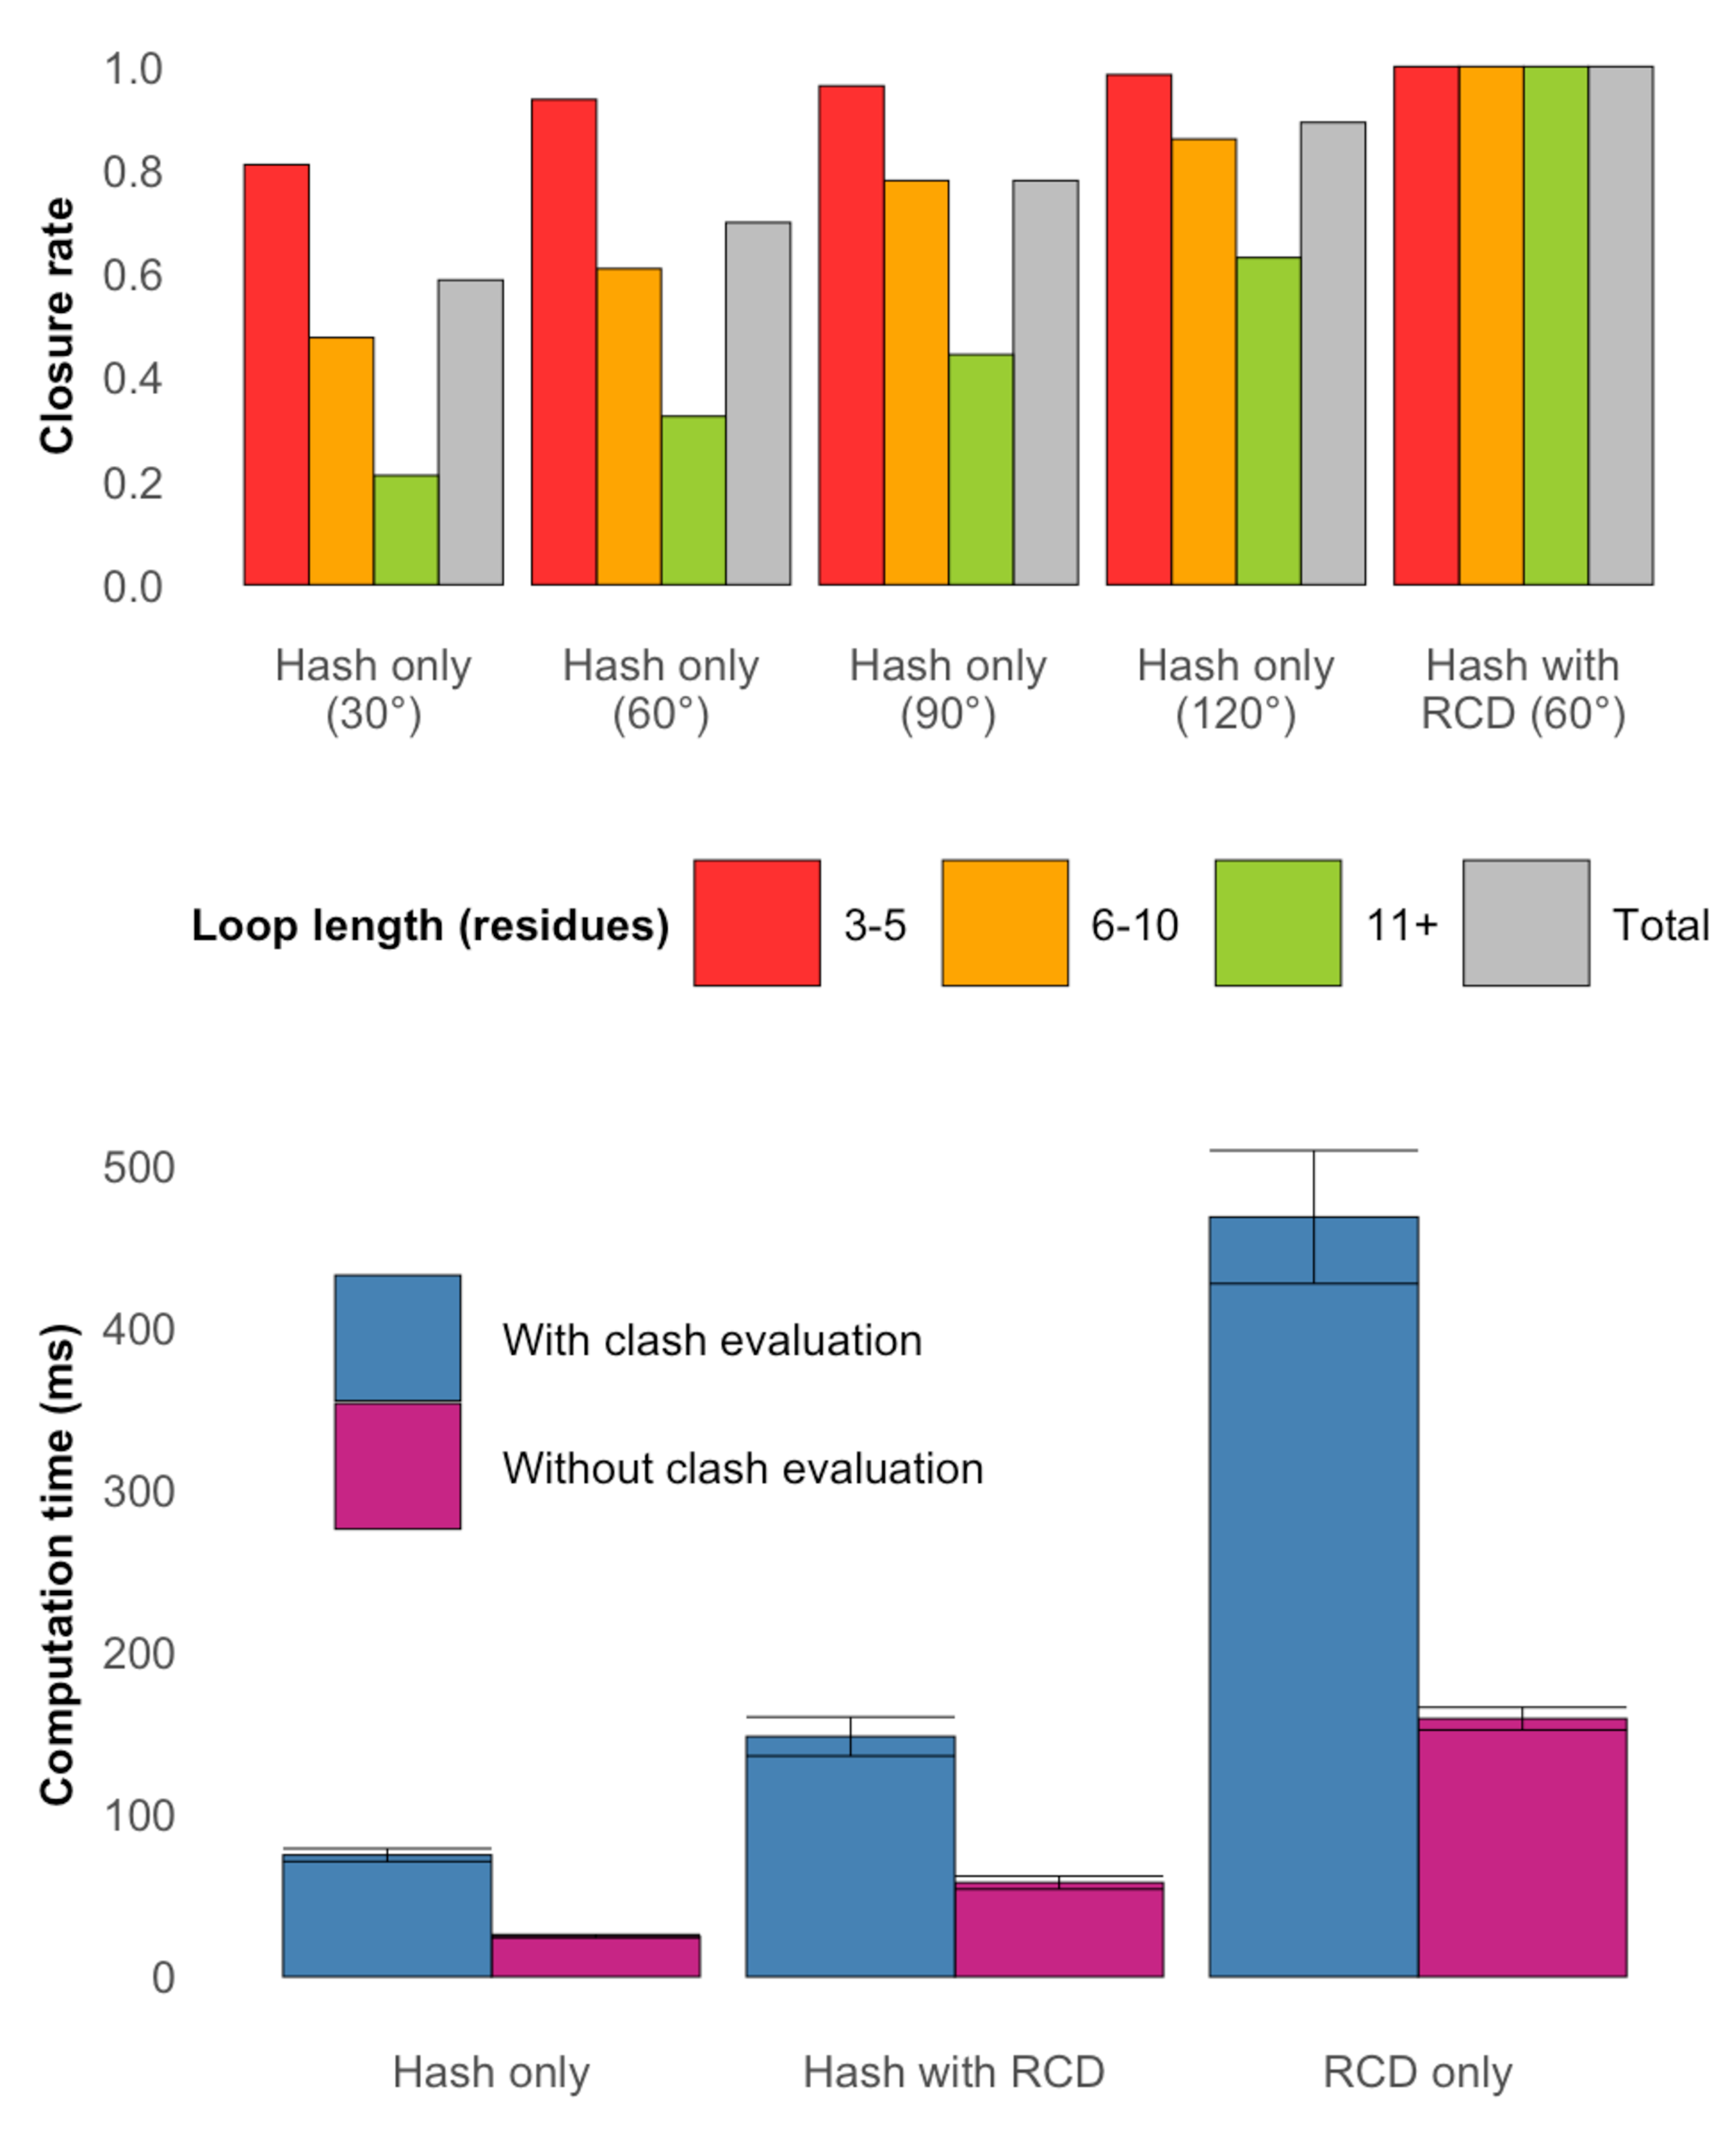
\includegraphics[width=3.25in]{Figures/loophash_closurerate.pdf}
 \caption[Evaluating conformational hashing and \gls{rcd} algorithms for loop construction.]{Evaluating conformational hashing and \gls{rcd} algorithms for loop construction. Top: The rotation angle bin width of the hash map influenced the loop closure rate of longer loops when using conformational hashing alone. When modeling short loops, we found high loop closure rates regardless of bin width. When conformational hashing was combined with \gls{rcd}, the loop closure rate increased to 100\% in our benchmark set. Bottom: The calculation of steric interference constituted the overwhelming majority of this algorithm's \gls{cpu} time requirement. Combining conformational hashing with \gls{rcd} was found to improve \gls{cpu} time efficiency.}
\label{fig:loophash_closurerate}
\end{wrapfigure}
 
\subsection{Conformational hashing achieves a high loop closure rate for short loops but RCD is required for long loops}

We evaluated the percentage of missing loop regions among our benchmark set (Table \ref{tab:loophash_benchmark}) that could be successfully constructed by first removing all non-terminal loop regions from each protein structure. We then constructed the missing loop regions using our algorithm and computed the loop closure rate per benchmark protein. This was performed with the original template library either prior to or following extension by template recombination and fragment-based loop construction (see section \ref{sec:loophash_methods}). In both cases, the loop libraries were binned at 60°.

When additional templates through fragment combination are excluded, the algorithm achieved a loop closure rate of 54\% over all twenty-nine benchmark proteins. As demonstrated above, a loop's length strongly influenced whether it could be successfully closed. For example, loops up to five residues long were successfully closed 87\% of the time, whereas loops ten residues long or greater were closed only 21\% of the time. By contrast, when the template library was extended to include loops generated using fragment-based construction, the overall loop closure rate could be improved by nearly 30\% to an overall closure rate of 70\% (Figure \ref{fig:loophash_closurerate}). Further increases in either the size of this library through additional fragment recombination did not appear to improve loop closure rate (data not shown). Nevertheless, as we mentioned above, following this step with \gls{rcd} achieved a closure rate of 100\%.
We found that Rosetta Loophash achieves a 99\% loop closure rate on the loops with a length of ten residues or less. However, this plummeted to 39\% when loop length exceeded ten residues. We note that this high loop closure rate is achieved in part by using a \SI{2}{\angstrom} bin width, which is wider than the \SI{1}{\angstrom} width used by Hash/RCD. A consequence of this approach is its reliance on optimization and refinement following the fitting, which increases the computational effort required (discussed below).

\subsection{CPU time requirement is dominated by the evaluation of steric interference}

Although the time complexity of the template look-up is O(1), the task of threading the target sequence against the template is O(n), which leads to linear time complexity for the overall loop construction algorithm. We therefore studied the effect this had on the CPU time required to execute the algorithm (specifically, the time between entering the \gls{mc} algorithm and leaving the \gls{mc} algorithm divided by the number of successfully constructed loop regions). To evaluate the contribution of the scoring term evaluating steric interference between residues relative to the overall CPU time requirement, the computation time needed by this term was evaluated separately. This was repeated for both \gls{rcd} alone and Hash/RCD.

When steric interference was not included during sampling, conformational hashing required on average 27±\SI{4}{ms} \gls{cpu} time per loop, whereas \gls{rcd} required 159±\SI{11}{ms}. By contrast, Hash/RCD required only 68±\SI{7}{ms} (Figure \ref{fig:loophash_closurerate}). When steric interference is calculated during sampling, the required CPU time increased to 59±5 ms for conformational hashing, 468±41 ms for RCD, and 161±13 ms for Hash/RCD. The evaluation of steric interferences dominated the computational burden by accounting for 54\%, 66\%, and 58\% of the total CPU time requirement among conformational hashing, \gls{rcd}, and Hash/RCD, respectively. Overall, these results demonstrate that using templates prior to coordinate descent can lead to a threefold decrease in the computation time of loop closure.

In contrast, the Rosetta Loophash protocol has a CPU runtime of \SI{160}{s} to sample each loop. This runtime is highly correlated with total protein size ($R^2=0.8$). We found that it is overwhelmingly devoted to minimization, as only 5\% of the algorithm's runtime involved conformational sampling.

\newpage

\subsection{Hash/RCD samples experimentally observed conformations}

Hash/RCD was developed to efficiently sample both major and minor populations that a loop might adopt. We assume that the experimentally determined structures deposited in the PDB correctly and accurately represent one of the proteins’ major populations (minor populations, by contrast, can only rarely be verified experimentally and are not considered for this benchmark). To test whether Hash/RCD correctly samples those conformations, we generated 100 models with constructed loop regions for each protein in the benchmark set. These conformations were subsequently compared to the experimentally determined structures using the \gls{rmsd} of the $\mathrm{C_{\upalpha}}$-atoms. For the membrane protein structure 3P5N, two non-terminal loops were not resolved in the X-ray-derived model and consequently excluded from this comparison. Moreover, in the case of homo-oligomeric proteins in the benchmark set, we excluded each instance of a given loop beyond the first to avoid their overrepresentation in the benchmark set. This led to 195 non-terminal loops comprised of three or more residues.

To focus on how effectively Hash/RCD could sample the major loop population, we determined the loop with the lowest $\mathrm{C_{\upalpha}}$ \gls{rmsd} among each of the 100 conformers sampled for each of the 195 loops in the benchmark set (Figure \ref{fig:loophash_rmsd}, top left). As expected, the lowest \gls{rmsd} among the conformers we sampled depended on the length of the loop, which in turn dictated the size of the sampling space. However, in the majority of loops, at least one conformer was within \SI{2}{\angstrom} of the experimentally observed structure, and all of the longer loops sampled at least one conformer within \SI{5}{\angstrom} $\mathrm{C_{\upalpha}}$ \gls{rmsd}. We found that these results were comparable to those obtained using \gls{rcd} alone, as well as the orthogonal hybrid method RosettaCM. In sharp contrast, Rosetta Loophash was far less capable of sampling native-like loop conformers with lengths exceeding ten residues. These results suggest that the lack of long templates prevents these loops from being closed using physiologically meaningful structures, and that sampling becomes the predominant obstacle for modeling long loops using conformational hashing.
 
\begin{figure}[h!]
\centering
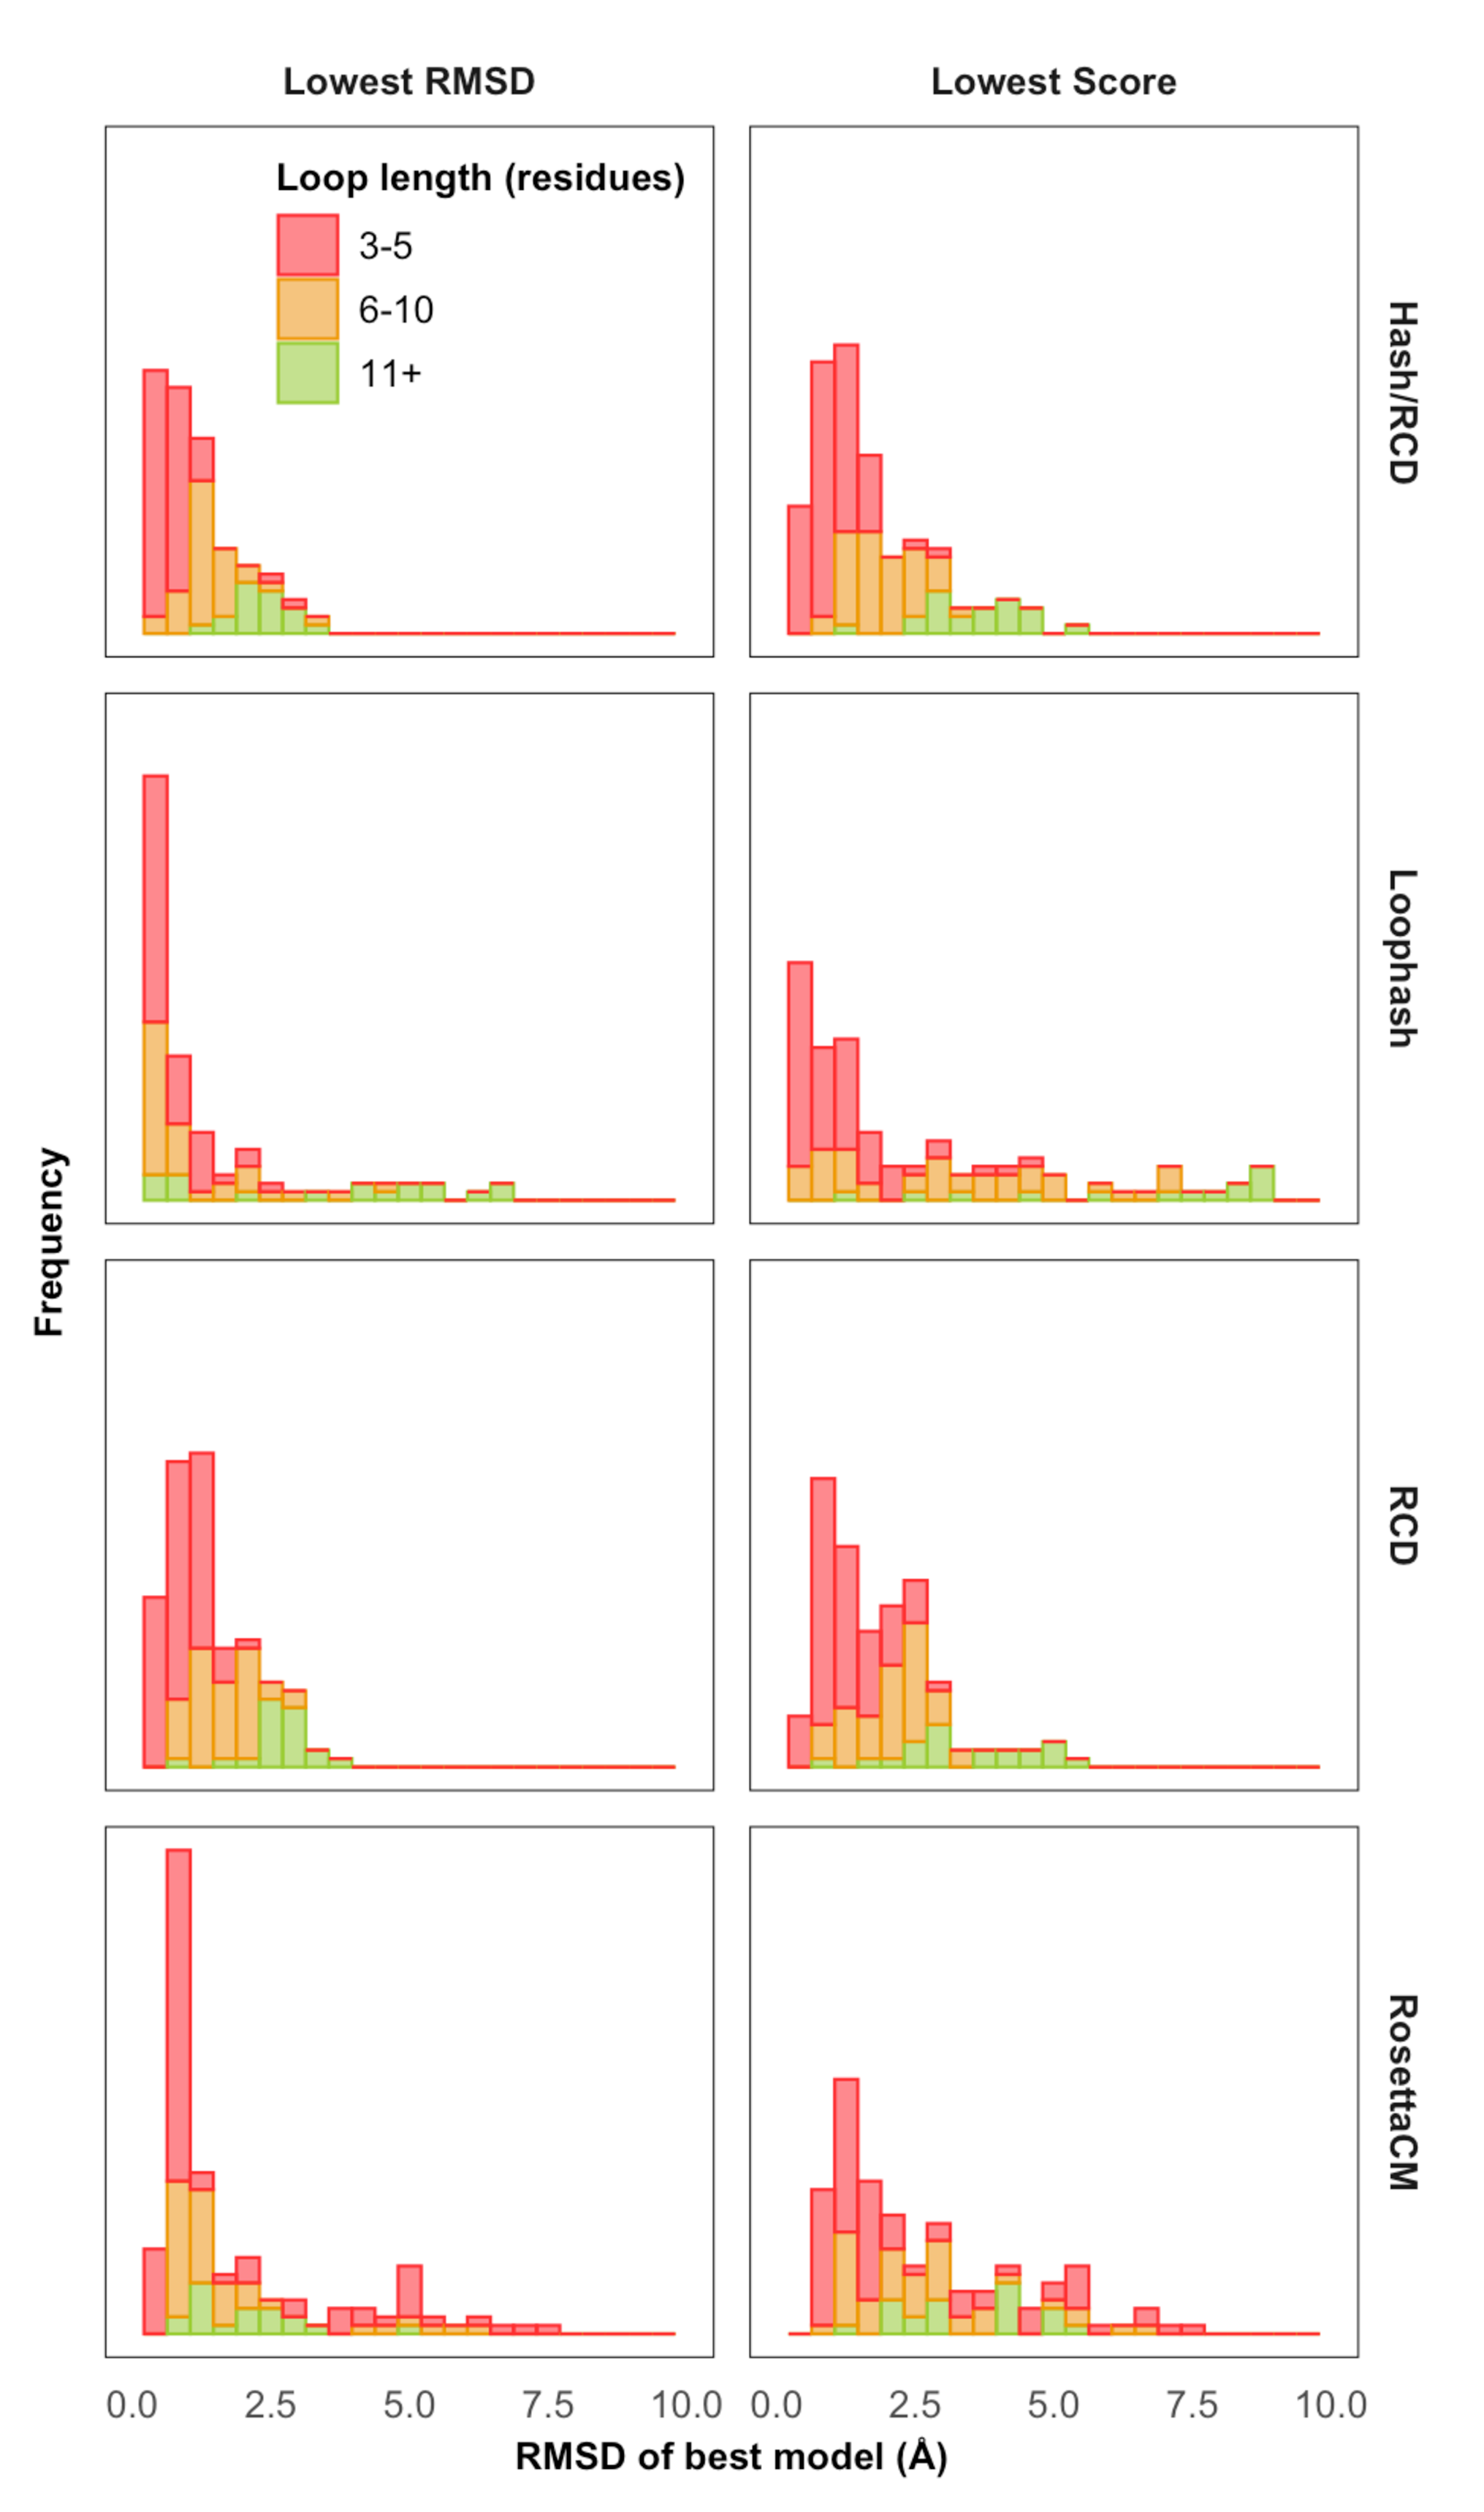
\includegraphics[width=3.25in]{Figures/loophash_rmsd.pdf}
 \caption[Loops generated using Hash/RCD are comparable in quality to those using RCD alone.]{Loops generated using Hash/RCD are comparable in quality to those using RCD alone. Left: Histograms of the lowest \gls{rmsd} values among loop conformers sampled by a variety of methods. Although Rosetta Loophash slightly outperformed Hash/RCD, \gls{rcd} alone, and RosettaCM when modeling short loops, it was unable to model native-like conformations for long loops. Right: Histograms of the \gls{rmsd} values of the lowest-scoring loop conformers.}
\label{fig:loophash_rmsd}
\end{figure}

When native loop conformations are unavailable and \gls{rmsd} values cannot be calculated, scoring functions must be used to infer which loop conformers are structurally relevant. We therefore focused on the lowest-scoring loops obtained using each method. Distributions are shown in Figure \ref{fig:loophash_rmsd} (right panels), and pairwise comparisons between Hash/RCD and other methods are shown in Figure \ref{fig:loophash_comparison}. The results reinforce the findings discussed above. Notably, the lowest-scoring loop conformer in most cases had \gls{rmsd} values only slightly higher than the lowest-\gls{rmsd} loop. We interpret this to suggest that the sampling space of the Hash/RCD method is focused on native-like conformers and ignores portions of the conformational space that are unlikely to be physiologically relevant. Moreover, these \gls{rmsd} values are comparable to those obtained from the lowest-scoring loops obtained using \gls{rcd} alone and contrast with the lowest-scoring conformers of long loops obtained by Rosetta Loophash. Finally, they improve upon loop modeling using RosettaCM, which interestingly was less effective at predicting short loops than we expected but reproduced the model quality of long loops that was observed using either Hash/RCD or \gls{rcd} alone.

Our results highlight the shortcomings of an exclusively template-based strategy when attempting to model long loops. When taken alongside the improvements in computation time, the results suggest that Hash/RCD arrives at conformations similar in quality to \gls{rcd} alone, but skips over a large number of intermediate conformations that would otherwise be expensive to sample. By further improving conformations obtained using conformational hashing, Hash/RCD achieves results comparable to \gls{rcd} alone on computational timescales comparable to those of template-based methods.

\newpage

\section{Discussion}

\begin{wrapfigure}{r}{0.4\textwidth}
\centering
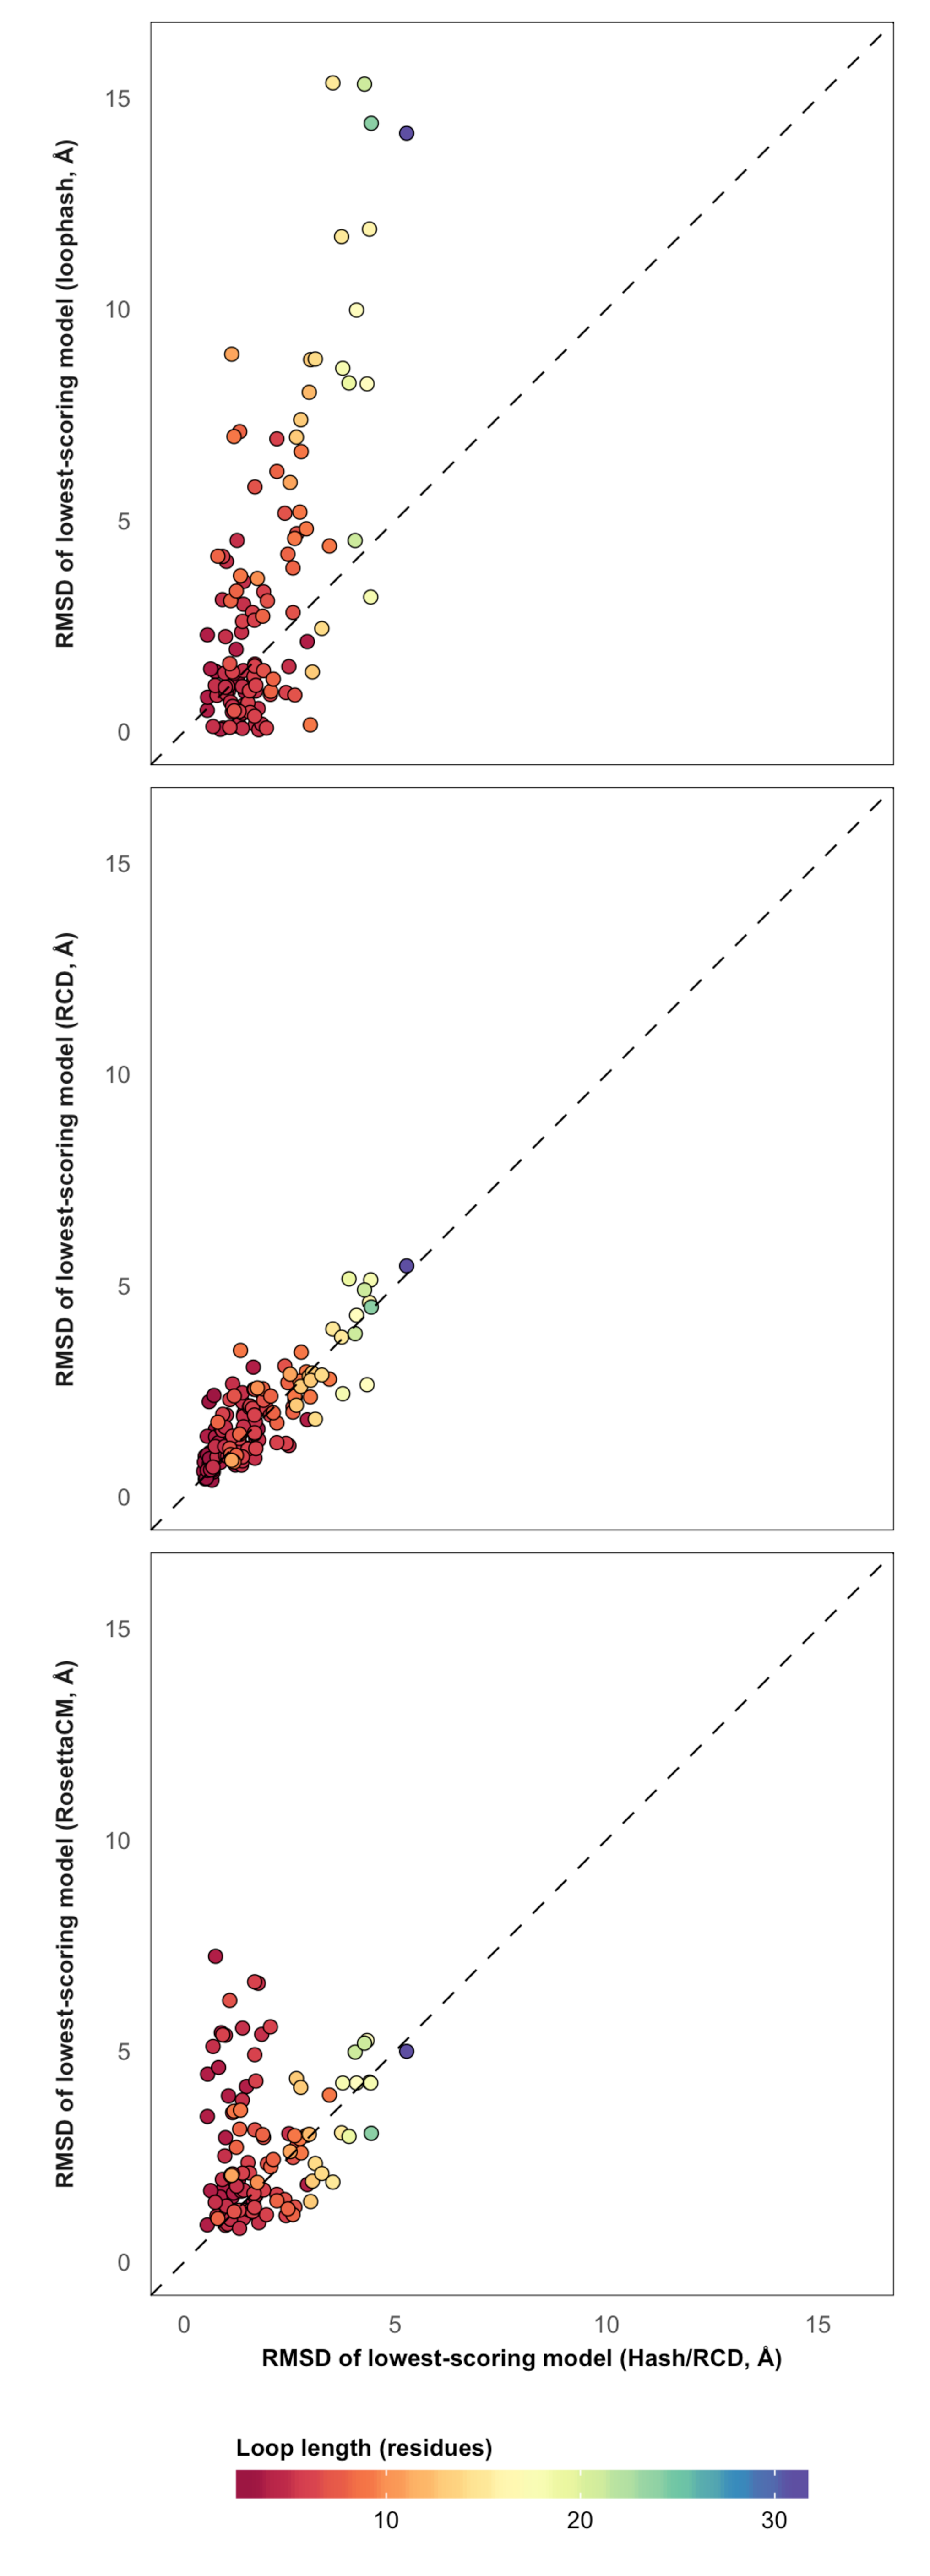
\includegraphics[width=2.35in]{Figures/loophash_comparison.pdf}
 \caption[Pairwise comparison of RMSD values among the best-scoring loop conformations obtained using Hash/RCD, Rosetta Loophash, RCD alone, or RosettaCM.]{Pairwise comparison of RMSD values among the best-scoring loop conformations obtained using Hash/RCD, Rosetta Loophash, RCD alone, or RosettaCM.}
\label{fig:loophash_comparison}
\end{wrapfigure}

\subsection{Complementing conformational hashing with template-independent modeling}

Loop modeling algorithms that employ conformational hashing methods must address the fact that most loops found in structures deposited in the PDB have sequence lengths of less than ten residues. This is evidenced by our initial loop library, which was derived from about 87,000 protein structures and disproportionately consists of short loops (Figure \ref{fig:loophash_db}). Additionally, longer loops can cover a larger conformational space, further impeding construction of long loops using conformational hashing. When we designed Hash/RCD, we found that this led to discrepancies between the loop closure rates for different loop lengths. For example, whereas loops between three to five residues long were closed 96\% of the time, the loop closure rate dropped to 61\% and 33\% among loops with lengths of either six to ten residues or eleven or more residues, respectively. (Figure 2). We mitigated this problem by using template recombination and fragment-based loop construction (see section \ref{sec:loophash_methods}), which improved the loop closure rate from 54\% to 70\%. Nonetheless, these results reinforced the need for template-independent conformational sampling. In this study, we integrated and applied an implementation of random coordinate descent to portions of loops that could not be constructed by conformational hashing, which compensated for the latter’s inability to close long loops. As a result, loop closure improved to 100\%. Consequently, whereas a stand-alone conformational hashing approach might suffice when the goal is to construct very short loop regions, loops found in most proteins will require a hybrid template-based/template-independent loop construction algorithm.

\subsection{Hash/RCD efficiently samples structurally diverse loop conformations}

Prediction of structural heterogeneity in proteins can be achieved by sampling diverse conformations (Figure \ref{fig:loophash_gallery}), which could capture major and minor populations of the protein in equilibrium. Random coordinate descent, although computationally demanding, achieves a high loop closure rate that cannot be replaced by more \gls{cpu}-efficient template-based methods. Relying on \gls{rcd} only in cases where conformational hashing was unsuccessful led to a significant reduction in \gls{cpu} time; this was demonstrated by a drop from 468ms using \gls{rcd} alone to \SI{161}{ms} using Hash/RCD (Figure \ref{fig:loophash_closurerate}). Thus, integrating conformational hashing with \gls{rcd} combines the efficiency of conformational hashing with the high loop closure rate of \gls{rcd}. The reduction in CPU time allows a wider range of possible loop conformations to be considered (Figure \ref{fig:loophash_comparison}). However, it needs to be noted that for longer loops in the benchmark set, the conformation of the experimentally determined structure was not sampled in any of the models to within \SI{2}{\angstrom} (Figure \ref{fig:loophash_rmsd}). Since this problem was exclusively faced by loops longer than ten residues in length, it can be solved by incorporating experimental data from technique such as electron paramagnetic resonance spectroscopy or fluorescence resonance energy transfer, to reduce the size of the conformational space. Alternatively, models obtained using Hash/RCD can be further refined in molecular dynamics simulations, which may save considerable sampling time and assist in identifying more physiologically relevant loop conformers.

\begin{figure}[h!]
\centering
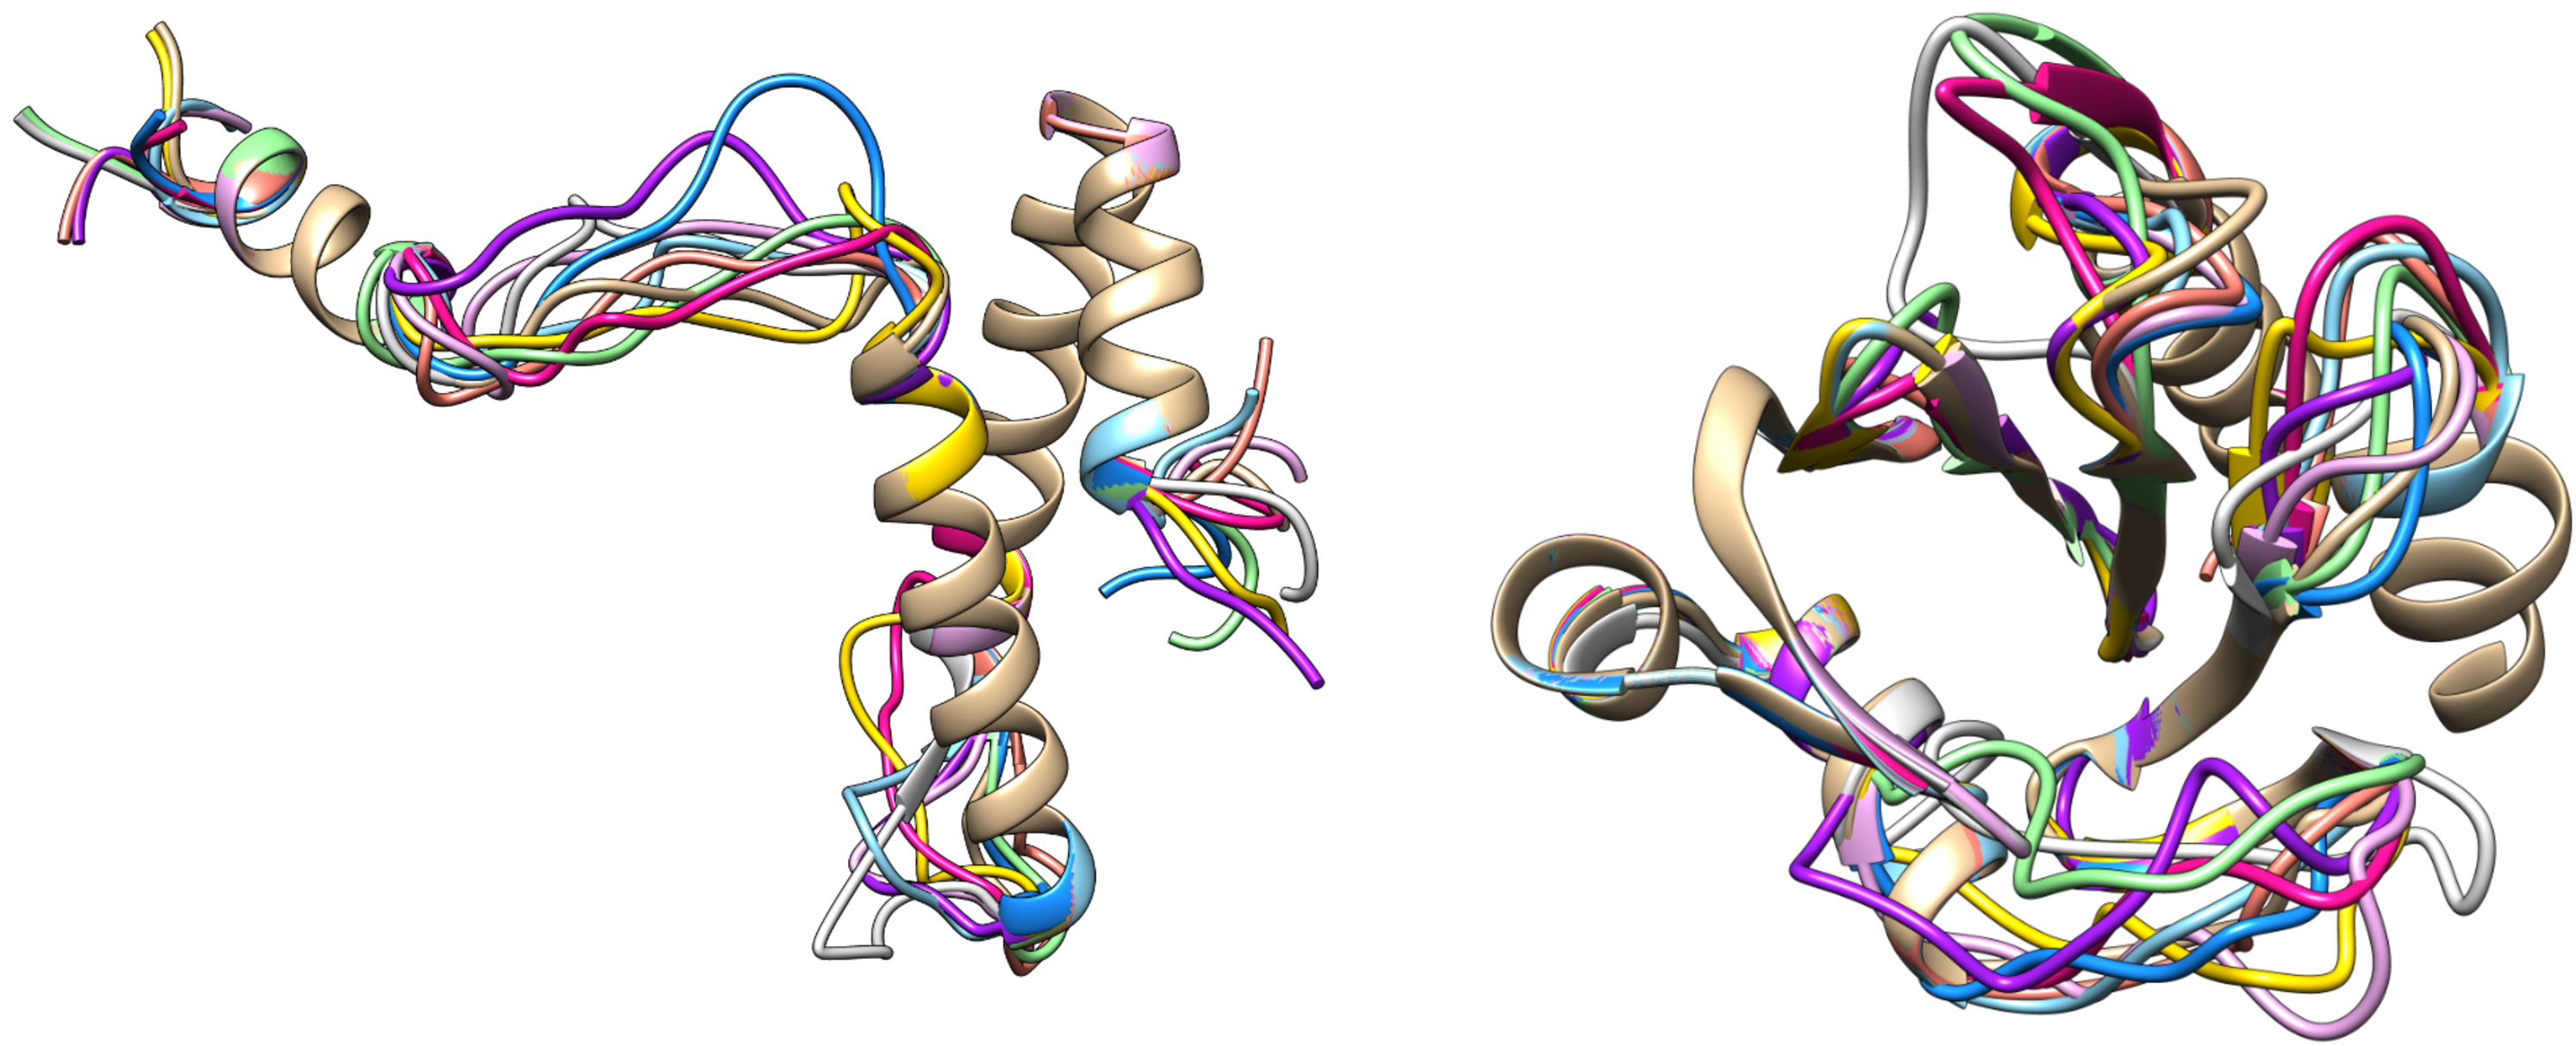
\includegraphics[width=5.5in]{Figures/loophash_gallery.pdf}
 \caption[Representative loop predictions obtained using Hash/RCD.]{Representative loop predictions obtained using Hash/RCD.}
\label{fig:loophash_gallery}
\end{figure}

\section{Conclusion}

The hybrid loop modeling method Hash/RCD provides an efficient way to sample structurally diverse loop conformations and is significantly faster than using the template-independent approach \gls{rcd} alone. We found that the constructed loop regions largely exhibit naturally occurring dihedral angles due to their construction from experimentally observed conformations. While this algorithm’s millisecond-timescale computation time was only quantified when implemented in the \gls{bcl}, we believe similar performance can be theoretically achieved in any protein structural modeling program.

Two applications of this approach are proposed. First, it could be used for the prediction of conformational ensembles in loop regions. For example, one could conceivably fit these loops against experimental data to determine a weighted distribution of conformers that represents the protein in question under equilibrium conditions. Second, the simultaneous prediction of adjacent loops could reveal a protein’s topological details, for example by capturing to what extent two loops may be intertwined. This may be relevant to multipass integral membrane proteins, as their solvent-exposed loop regions are least likely to be resolved.

\section{Acknowledgments}

We want to thank Dr. Marion F. Sauer for thorough proofreading of this manuscript. Work in the Meiler laboratory is supported through NIH (R01 GM080403 and R01 GM073151). The authors acknowledge funding by the Deutsche Forschungsgemeinschaft (DFG, German Research Foundation) through SFB1423, project number 421152132, subproject A07 and Z04. Parts of the data analysis were performed using R in conjunction with the ggplot2 package \citep*{Wickham2009}. Figures depicting protein models were created using Chimera \citep*{Pettersen2004} and composite figures were created using Inkscape. To determine sequence identities between the template set and the benchmark set, the sequences were aligned using Clustal Omega \citep*{Sievers2011}.

